\documentclass{beamer}

\mode<presentation>
{
  \usetheme{Boadilla}
  % possiblities Singapore, Malmoe, Dresden 
  \setbeamercovered{transparent}
}

%\setbeamertemplate{navigation symbols}{} 
% removes the navigation symbols

%color setting more or less matching U of A colors
\setbeamercolor*{palette secondary}{use=structure,fg=white,bg=structure.fg!55!black}
\setbeamercolor*{palette tertiary}{use=structure,fg=white,bg=red!50!black}

\usepackage[english]{babel}
\usepackage{tikz}
\usepackage[utf8]{inputenc}
\usepackage[T1]{fontenc}
\usepackage{graphicx}
\usepackage{amsfonts}
\usetikzlibrary{shapes.geometric}

\title[TPS free energies]{Transition path sampling and the calculation of free energies of enzymatic reactions}
\subtitle{} 

\author[Schwartz Group]{Sree Ganesh Balasubramani}

\institute[U of A]{Schwartz Group \\ Chemistry and Biochemistry \\ University of Arizona}
\date{}

% If you wish to uncover everything in a step-wise fashion, uncomment
% the following command: 
%\beamerdefaultoverlayspecification{<+->}
\begin{document}
%------------------------------------------------------------------------------
\begin{frame}
  \titlepage
\end{frame}
%------------------------------------------------------------------------------
\begin{frame}
  \frametitle{Features of beamer}
\begin{itemize}
\item Complicated, elegant templates
\item Viewers can see the progress of the presentation
\item Nice boxes for theorems, definitions, etc.
\item Easy to use once you know LaTex
\item With extra options and goodness comes complication
\end{itemize}
\end{frame}
%------------------------------------------------------------------------------
\begin{frame}
\frametitle{Transition path sampling (TPS)}
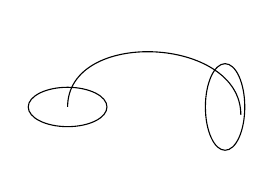
\begin{tikzpicture}
 \draw (3,2) ellipse (.5cm and .25cm);
 \draw (5,2) ellipse (.25cm and .55cm);
\draw (5.2,1.9) to [controls=+(90:1) and +(90:1)] (3,2);
\end{tikzpicture} 
\begin{tikzpicture}[
node distance = 3mm and 9mm,
% block/.style = {rectangle, draw, minimum height=22mm},
 ellip/.style = {draw, ellipse, align=center},
                    ]
%\node (n1) [block] {block};
\node (n2) [ellip, above right=of n1.east]  {longer text\\ in two lines};
\node (n3) [ellip, below right=of n1.east]  {short\\ text};
    \end{tikzpicture}
\end{frame}
%------------------------------------------------------------------------------
%\input{BeamerIntro.tex}
%\input{BeamerOverlays.tex}
%\input{funmath.tex}
%\input{BeamerConcl.tex}

\end{document}